\chapter{Set up}
The stretcher set up contains the following components, visible in figure \ref{fig:setup}.

\begin{itemize}
	\item The stretcher frame with the two stages, number 1 in the picture and a load cell.
	\item Two USB-to-Serial converter, number 2 and 3, to connect the stages with the laptop.
	\item A analog/digital converter for the load cell, number 4 in the picture.
	\item A power supply for the analog/digital converter, number 5 in the picture.
	\item A USB-to-Serial converter, number 6, to connect the analog/digital converter with the laptop.
	\item A laptop with the installed stretcher software.
\end{itemize}

\begin{figure}[!ht]
	\centering
		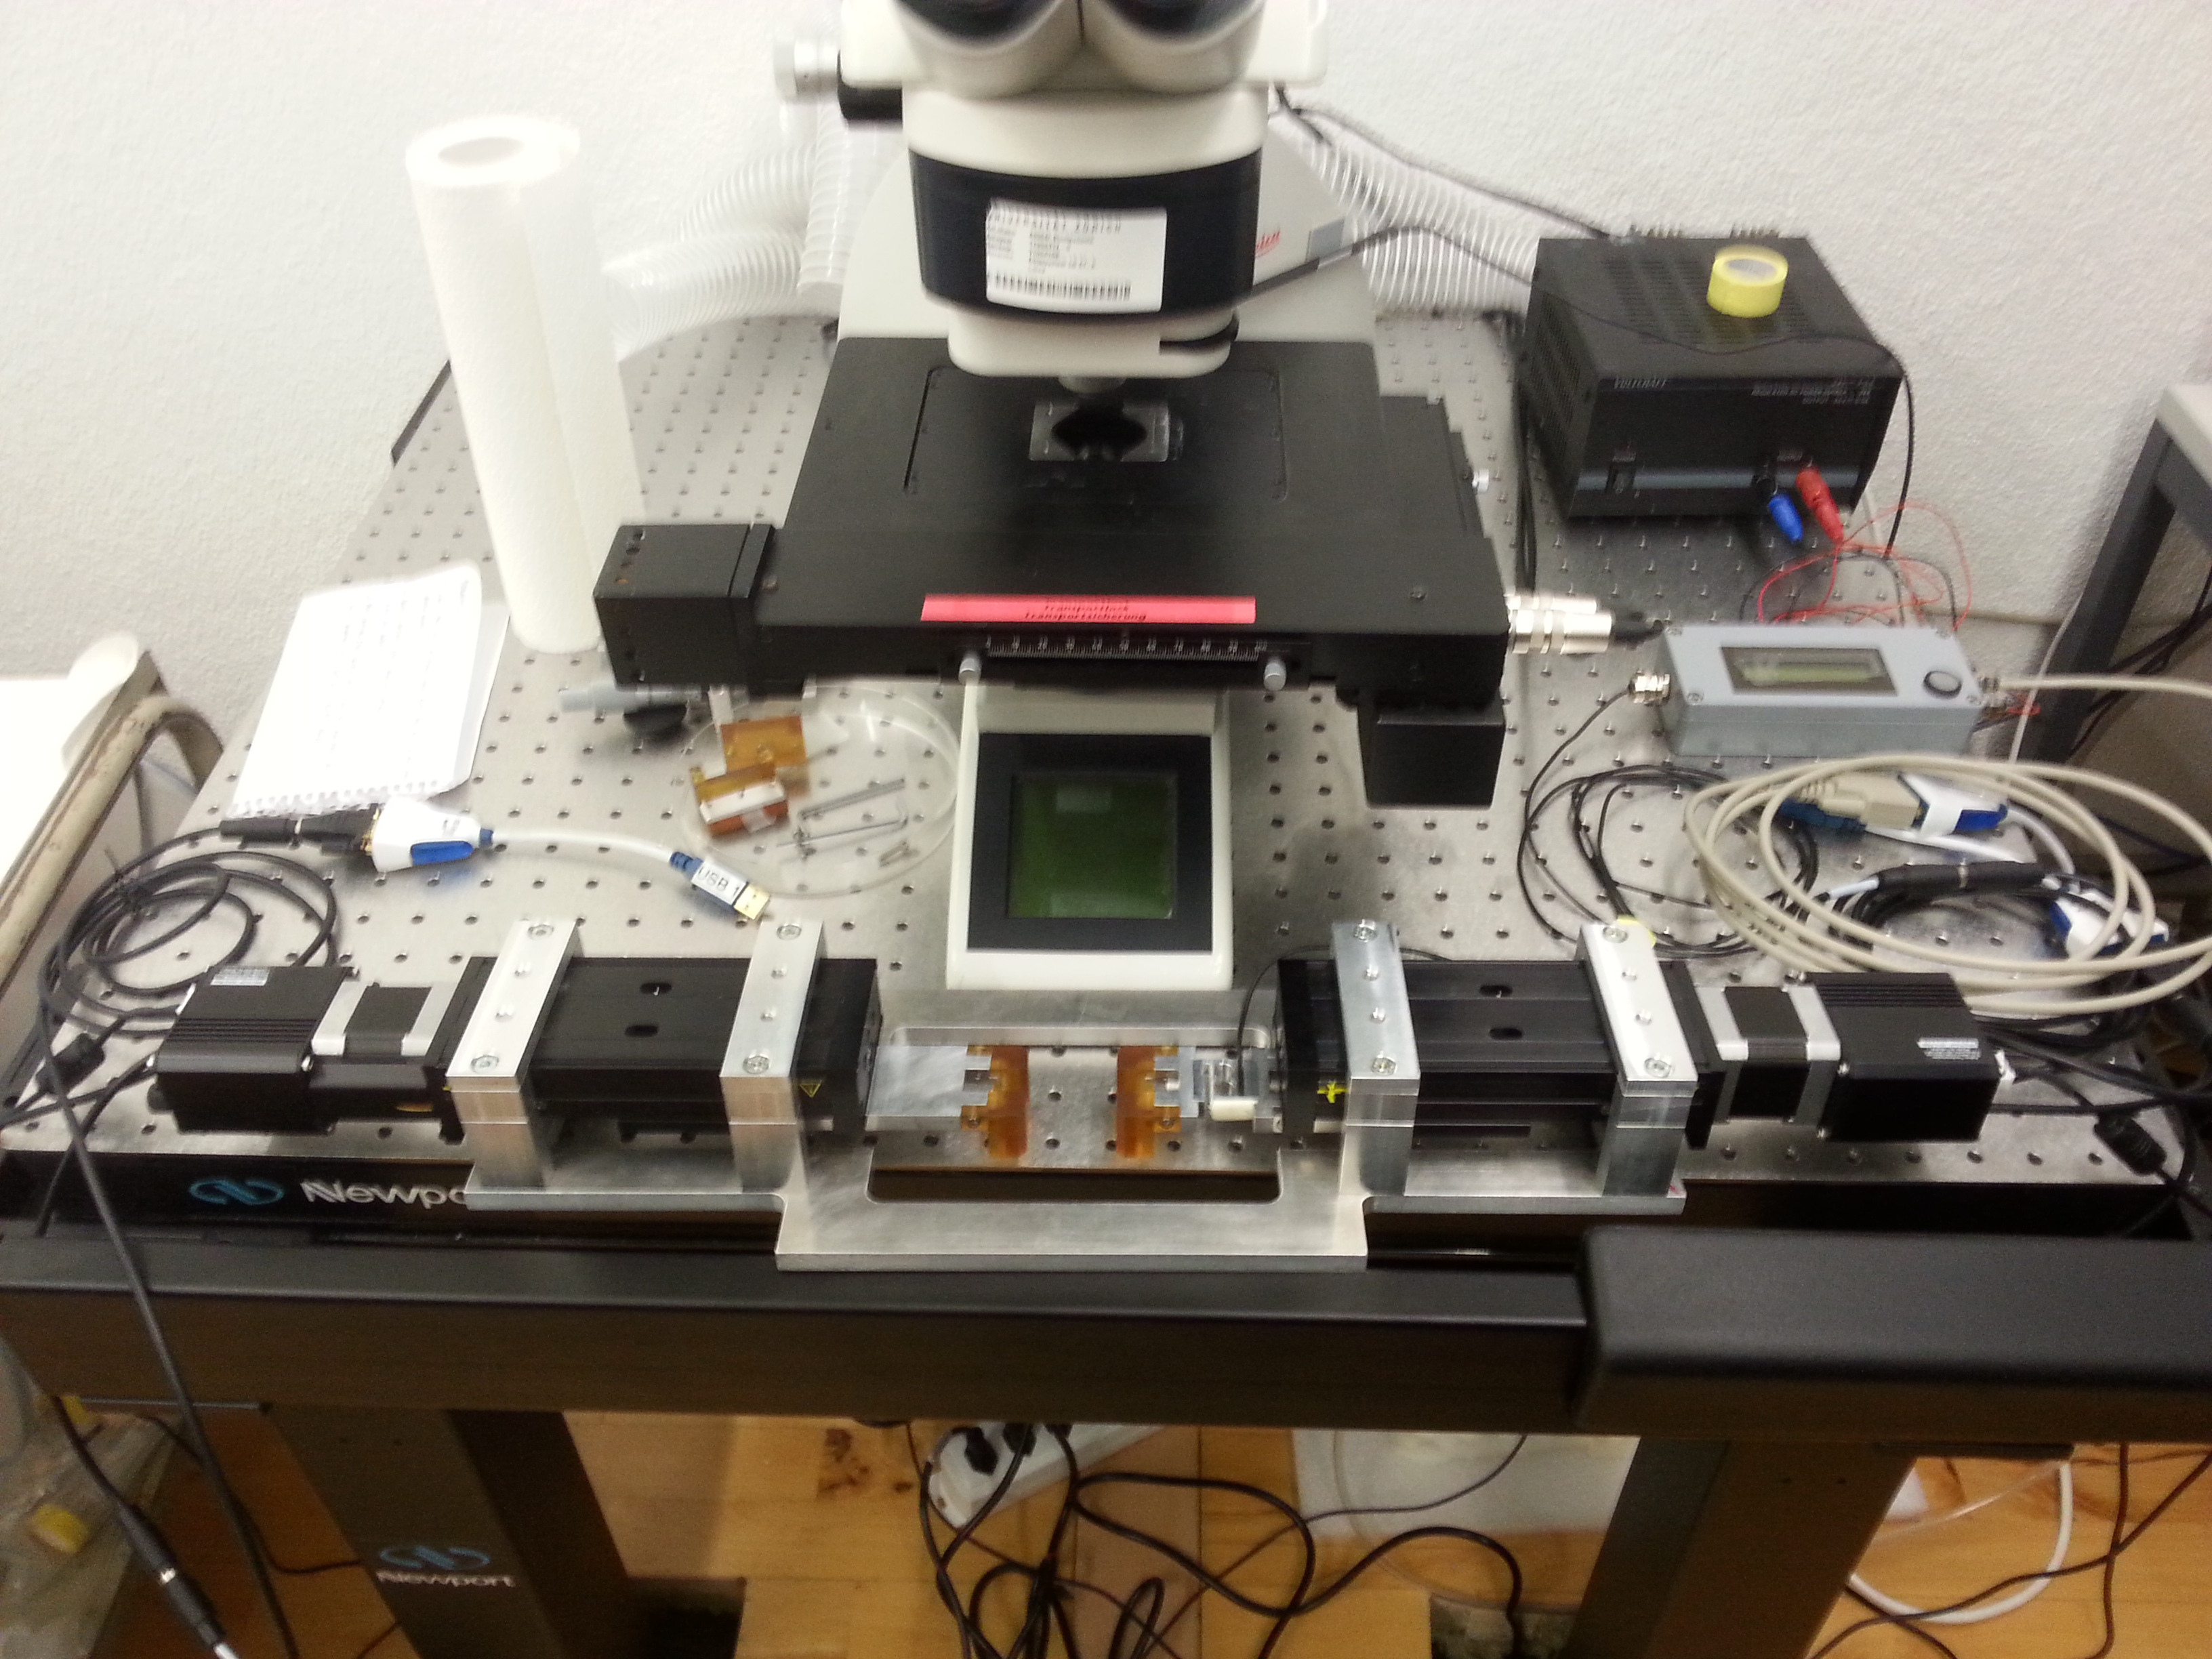
\includegraphics[width=1.0\textwidth]{images/SetUp}
	\caption{Set up}
	\label{fig:setup}
\end{figure}

If the whole system is not in use for longer time, it is recommended, to unplug the power supply of the stages, shown in figure \ref{fig:powersupply} and the power supply of the load cell.
\\

\begin{figure}[!ht]
	\centering
		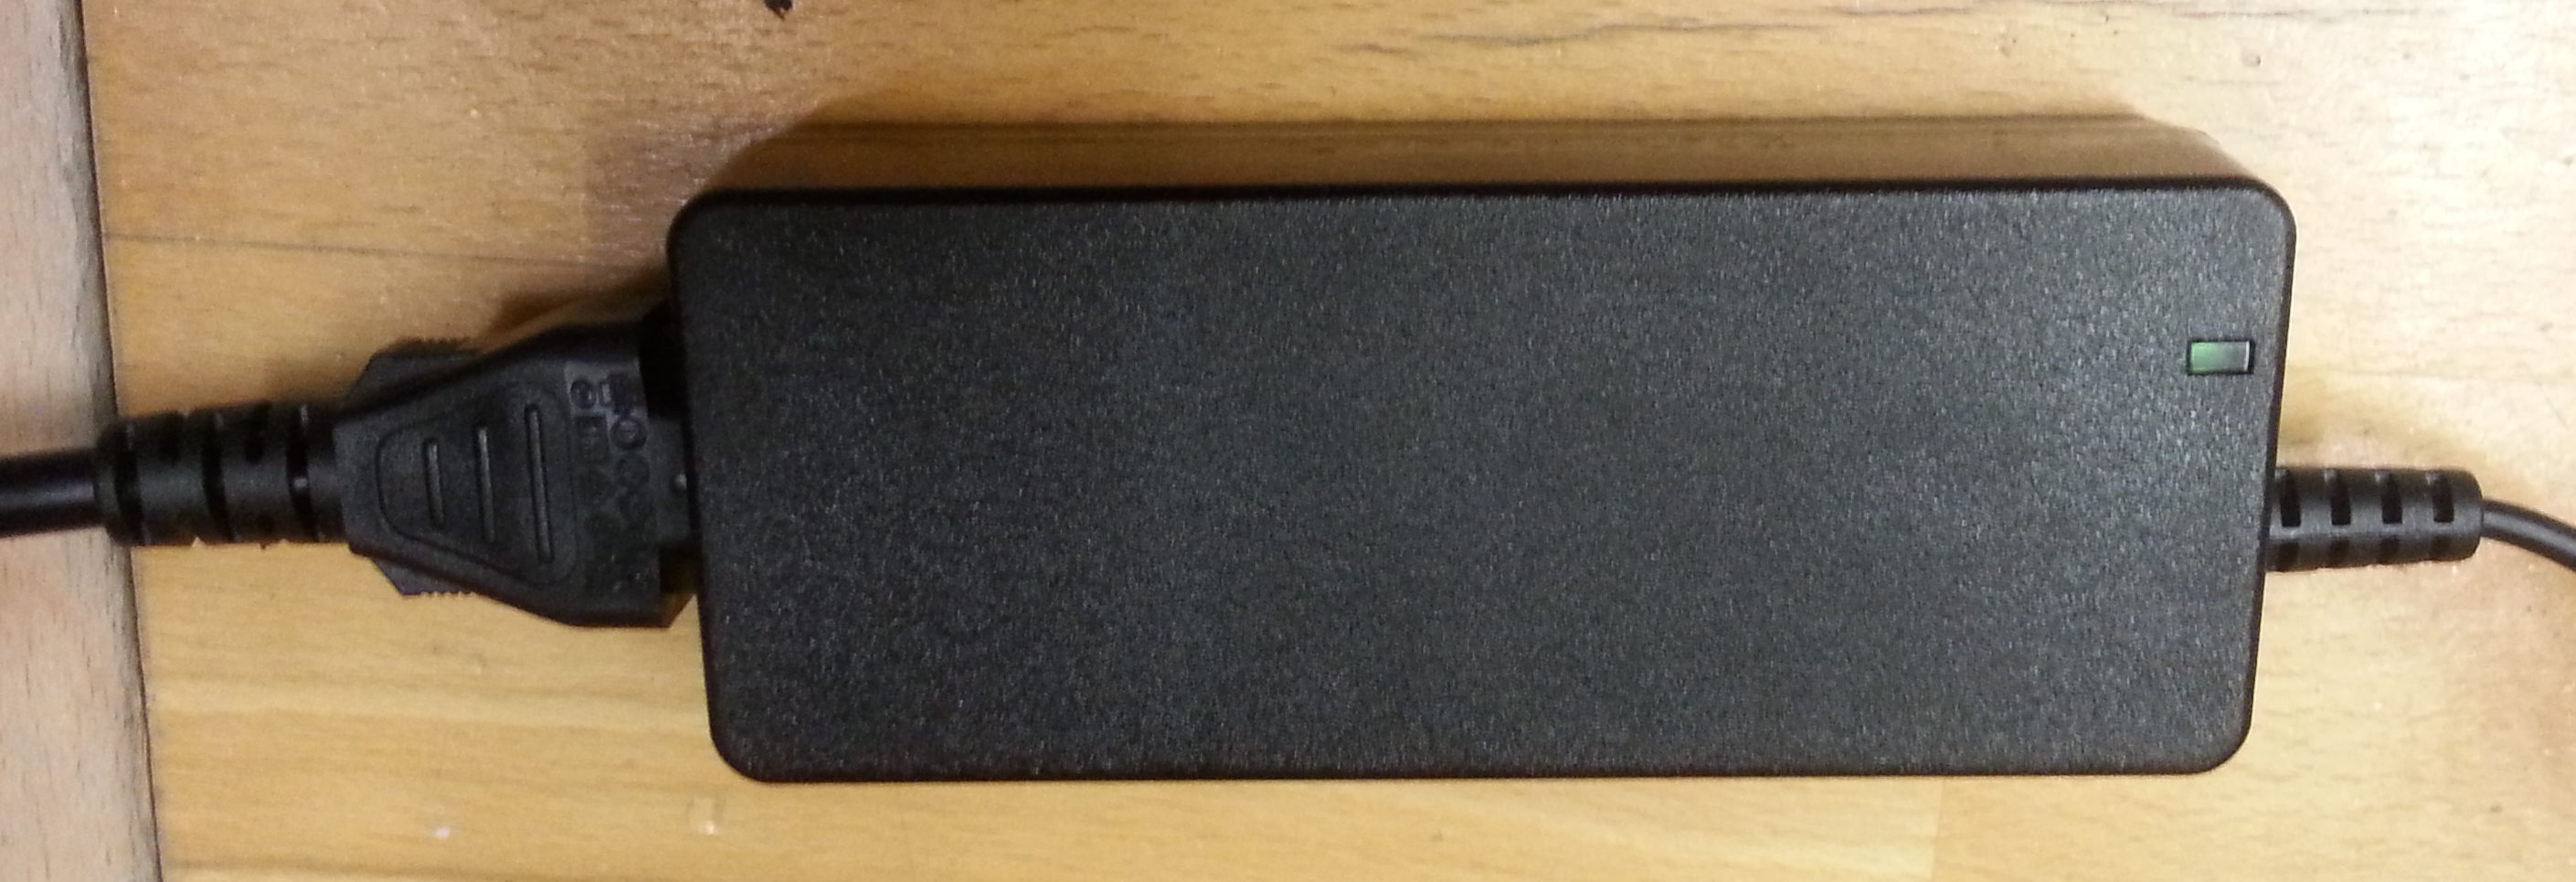
\includegraphics[width=1.0\textwidth]{images/PowerSupply}
	\caption{Power supply of a stage}
	\label{fig:powersupply}
\end{figure}

When the whole system is started, it is recommended, to wait until the measurement values on the analog/digital converter are visible as shown in figure \ref{fig:analogdigitalconverter}. It is also a good practice to wait around 15 minutes until the analog/digital converter warmed up and shows more or less stable force values before starting with experiments. After that, the values can be zeroed by pushing the button on the analog/digital converter.

\begin{figure}[!ht]
	\centering
		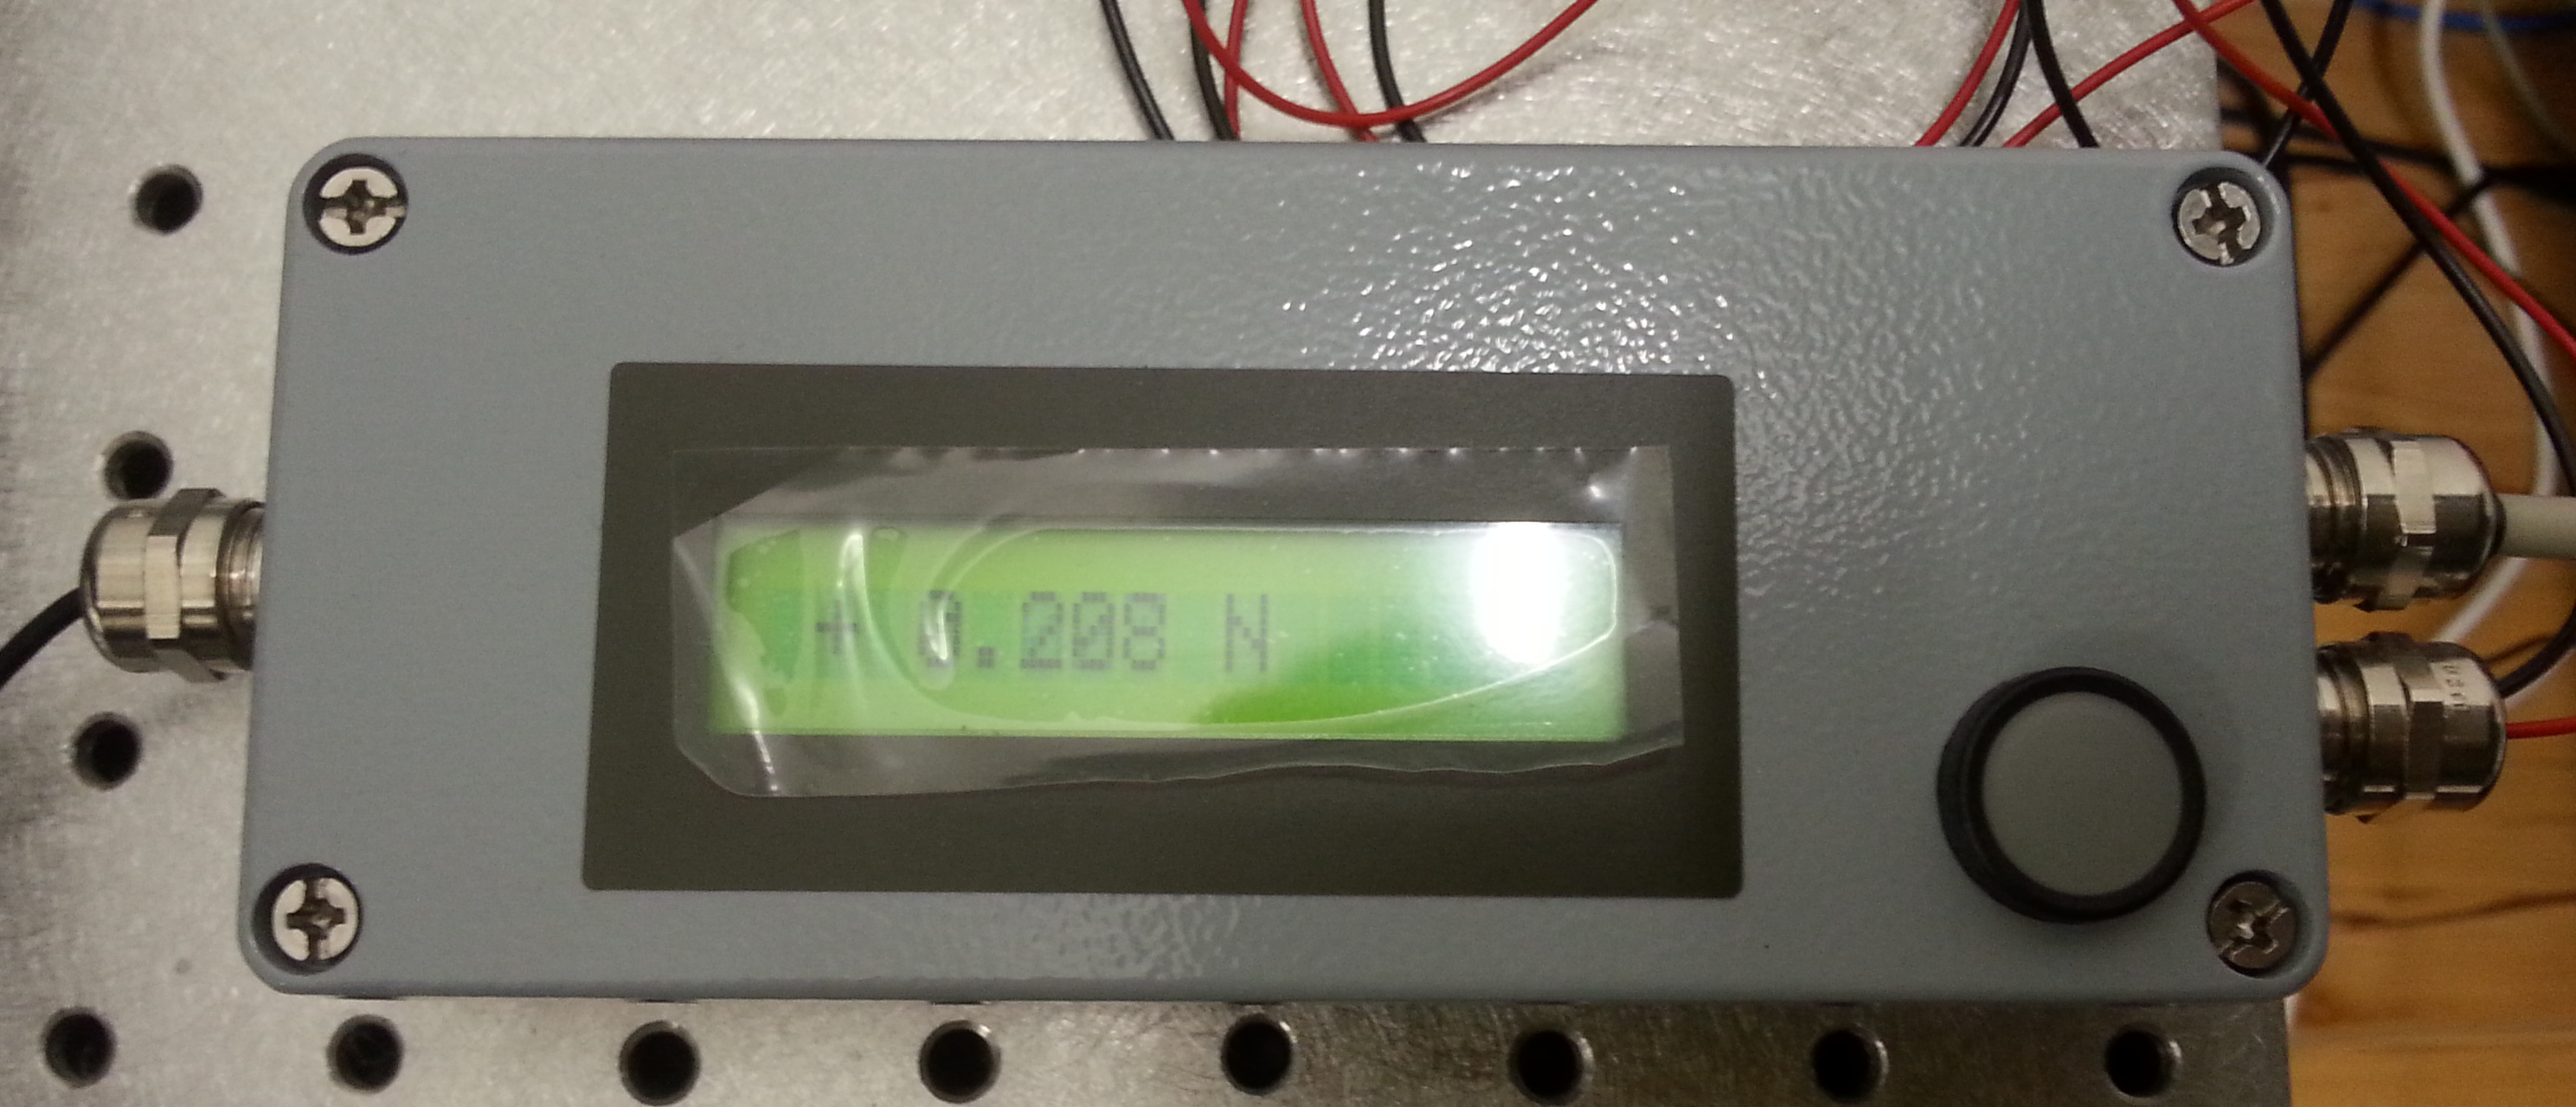
\includegraphics[width=1.0\textwidth]{images/AnalogDigitalConverter}
	\caption{The analog/digital converter of the load cell}
	\label{fig:analogdigitalconverter}
\end{figure}
